\documentclass[border=3pt]{standalone}
\usepackage{amsmath}\usepackage{amssymb}
\usepackage{fontspec}\setsansfont{Arial}\renewcommand{\familydefault}{\sfdefault}
\usepackage{tikz}
\usetikzlibrary{arrows.meta,positioning,calc,fit,backgrounds,shapes.geometric}
\definecolor{titlegray}{HTML}{5F6B78}\definecolor{ent}{HTML}{7B8794}
\definecolor{fo}{HTML}{5AA9C4}\definecolor{ho}{HTML}{2E6B86}
\definecolor{inf}{HTML}{D98A3D}\definecolor{vio}{HTML}{9B86C4}
\definecolor{smac}{HTML}{2E8AA6}\definecolor{kgc}{HTML}{E7B15A}
\definecolor{fillteal}{HTML}{E3EEF2}\definecolor{fillamber}{HTML}{FBF0E2}
\definecolor{fillgrey}{HTML}{F1F3F5}\definecolor{fillviolet}{HTML}{EFEAF6}
\definecolor{inkmid}{HTML}{3D4751}\definecolor{distract}{HTML}{B3403A}
\begin{document}
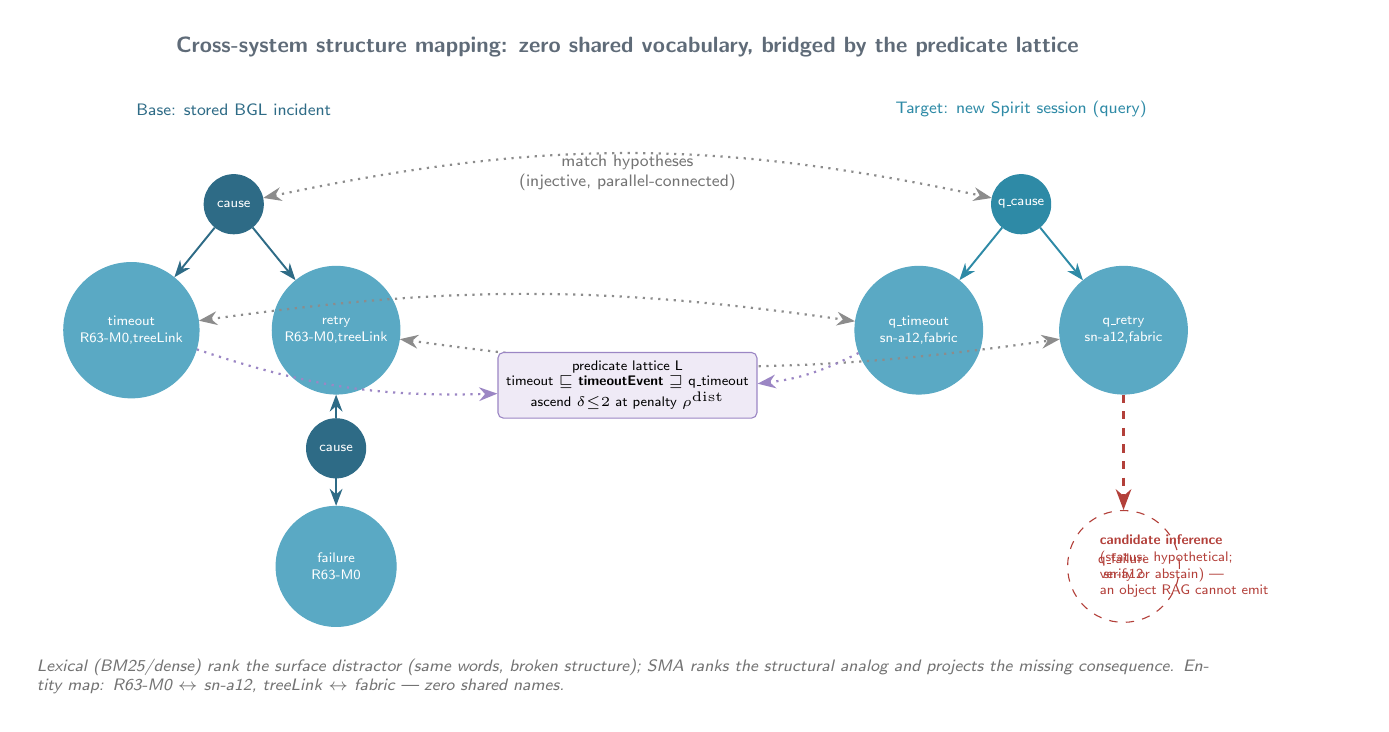
\begin{tikzpicture}[
  font=\sffamily,>=Stealth,
  ttl/.style={font=\sffamily\fontsize{8}{9}\selectfont\bfseries, color=titlegray, align=center},
  sub/.style={font=\sffamily\fontsize{6}{7}\selectfont, color=black!55, align=center},
  micro/.style={font=\sffamily\fontsize{5.2}{6}\selectfont, color=black!50, align=center},
  enode/.style={circle, draw=ent, fill=ent, text=white, font=\sffamily\fontsize{5.2}{6}\selectfont, inner sep=0pt, minimum size=6.5mm, align=center},
  fnode/.style={circle, draw=fo, fill=fo, text=white, font=\sffamily\fontsize{5.2}{6}\selectfont, inner sep=0pt, minimum size=7mm, align=center},
  hnode/.style={circle, draw=ho, fill=ho, text=white, font=\sffamily\fontsize{5.2}{6}\selectfont, inner sep=0pt, minimum size=7.5mm, align=center},
  pbox/.style={rounded corners=2pt, draw, align=center, inner sep=3pt, font=\sffamily\fontsize{6}{7}\selectfont},
  flowarr/.style={->, line width=0.7pt, color=black!55},
  horel/.style={->, line width=0.7pt, color=ho},
  forel/.style={->, line width=0.6pt, color=fo!80},
]

\node[ttl] at (8,7.0) {Cross-system structure mapping: zero shared vocabulary, bridged by the predicate lattice};
\node[sub,color=ho] at (3,6.2) {Base: stored BGL incident};
\node[sub,color=smac] at (13,6.2) {Target: new Spirit session (query)};
% base DAG (left)
\node[hnode] (bh1) at (3,5.0) {cause};
\node[fnode,text width=1.6cm,inner sep=1pt,minimum size=0pt] (bt) at (1.7,3.4) {\fontsize{4.6}{5.4}\selectfont timeout\\R63-M0,treeLink};
\node[fnode,text width=1.5cm,inner sep=1pt,minimum size=0pt] (br) at (4.3,3.4) {\fontsize{4.6}{5.4}\selectfont retry\\R63-M0,treeLink};
\node[hnode] (bh2) at (4.3,1.9) {cause};
\node[fnode,text width=1.4cm,inner sep=1pt,minimum size=0pt] (bf) at (4.3,0.4) {\fontsize{4.6}{5.4}\selectfont failure\\R63-M0};
\draw[horel] (bh1)--(bt); \draw[horel] (bh1)--(br); \draw[horel] (bh2)--(br); \draw[horel] (bh2)--(bf);
% target DAG (right) - disjoint vocabulary
\node[hnode,draw=smac,fill=smac] (th1) at (13,5.0) {q\_cause};
\node[fnode,fill=fo,text width=1.5cm,inner sep=1pt,minimum size=0pt] (tt) at (11.7,3.4) {\fontsize{4.6}{5.4}\selectfont q\_timeout\\sn-a12,fabric};
\node[fnode,fill=fo,text width=1.5cm,inner sep=1pt,minimum size=0pt] (tr) at (14.3,3.4) {\fontsize{4.6}{5.4}\selectfont q\_retry\\sn-a12,fabric};
\node[circle,draw=distract,dashed,fill=white,text=distract,text width=1.3cm,inner sep=1pt,minimum size=10mm,font=\sffamily\fontsize{4.6}{5.4}\selectfont,align=center] (tf) at (14.3,0.4) {q\_failure\\sn-a12};
\draw[horel,color=smac] (th1)--(tt); \draw[horel,color=smac] (th1)--(tr);
% candidate inference projection
\draw[->,dashed,line width=1pt,color=distract] (tr)--(tf);
\node[micro,color=distract,align=left,text width=3.2cm] at (15.6,0.4) {\textbf{candidate inference}\\(status: hypothetical;\\verify or abstain) ---\\an object RAG cannot emit};
% correspondences (bundled)
\draw[<->,dotted,line width=0.8pt,color=black!45] (bh1) to[bend left=12] (th1);
\draw[<->,dotted,line width=0.8pt,color=black!45] (bt) to[bend left=8] (tt);
\draw[<->,dotted,line width=0.8pt,color=black!45] (br) to[bend right=8] (tr);
\node[sub,align=center] at (8,5.4) {match hypotheses\\(injective, parallel-connected)};
% lattice ascension inset
\node[draw=vio,fill=fillviolet,rounded corners=2pt,align=center,inner sep=3pt,font=\sffamily\fontsize{4.8}{5.6}\selectfont] (lat) at (8,2.7) {predicate lattice L\\ timeout $\sqsubseteq$ \textbf{timeoutEvent} $\sqsupseteq$ q\_timeout\\ ascend $\delta{\le}2$ at penalty $\rho^{\mathrm{dist}}$};
\draw[->,dotted,line width=0.8pt,color=vio] (bt) to[bend right=10] (lat);
\draw[->,dotted,line width=0.8pt,color=vio] (tt) to[bend left=10] (lat);
% bottom contrast strip
\node[sub,align=left,text width=15cm] at (8,-1.0) {\textit{Lexical (BM25/dense) rank the surface distractor (same words, broken structure); SMA ranks the structural analog and projects the missing consequence. Entity map: R63-M0 $\leftrightarrow$ sn-a12, treeLink $\leftrightarrow$ fabric --- zero shared names.}};

\end{tikzpicture}
\end{document}
